\documentclass[aspectratio=169]{beamer}

\usetheme{metropolis}
\title{MORR: Product presentation}
\author{Irma Suppes, Karl Rubel, Mingyi Li, Niklas Bülow, Sönke Jendral}
\date{26th of March, 2020}
\institute{KIT / Teco}
\begin{document}
  \maketitle
  
  \begin{frame}{MORR}
      Medical Online Research Recorder
  \end{frame}

  \section{Our Mission}

  \begin{frame}{Our Mission}
  	Recording a broad variety of user interactions in medical research to enable data scientists to perform target page prediction.
  \end{frame}

  \section{Our Product}
  
   \subsection{Our Goals}
   
   \begin{frame}
       Collecting rich and meaningful data!
   \end{frame}
   
   \begin{frame}{Collecting rich and meaningful data!}
        \begin{itemize}
            \item Desktop Video Capture
            \item Clipboard: cut, copy, paste
            \item Keyboard: key presses and modifiers
            \item Mouse: mouse clicks, movement and scroll wheel interactions
            \item Window management: window focus, movement, resizing, state changes
            \item Web browser: button click, tab open/close/switch, file download, hover, navigation, text input and selection
        \end{itemize}
   \end{frame}
   
   \subsection{Modular Expandability}
   \begin{frame}
       Extensible and scalable application!
   \end{frame}
   
   \begin{frame}{Extensible and scalable application!}
   		\begin{itemize}
            \item Modules encapsulate logic for collecting data.
            \item MEF (Managed Extensibility Framework) allows to load modules and additional local packages.
            \item Allow extending the scope of data collection by other developers, through well defined interfaces.
    	\end{itemize}
   \end{frame}
   
   \begin{frame}
   		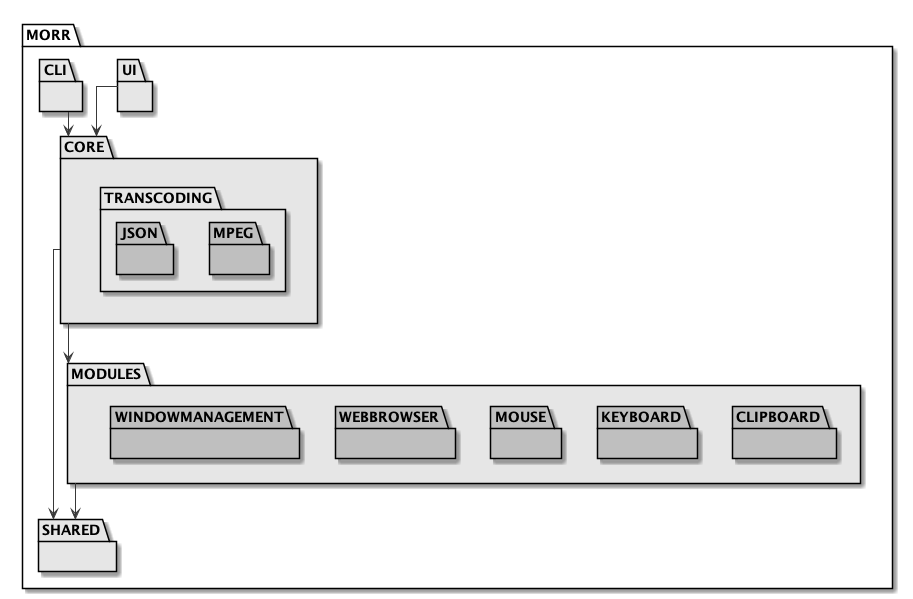
\includegraphics[width=0.8\linewidth]{resources/AllPackages.png}
   \end{frame}
   
   \subsection{Configurability}
   \begin{frame}{Configurability}
       Sometimes, fewer or more types of user interactions are focused during target page prediction and some components of our application require user-defined parameters.
   \end{frame}
   
   \begin{frame}{Configurability}
   		Configuration File allows to modify broad range of settings:
   		\begin{itemize}
			\item Enabled Modules
			\item Module specific configuration
			\item Decoder and Encoder configuration
		\end{itemize}
   \end{frame}
   
   \begin{frame}
		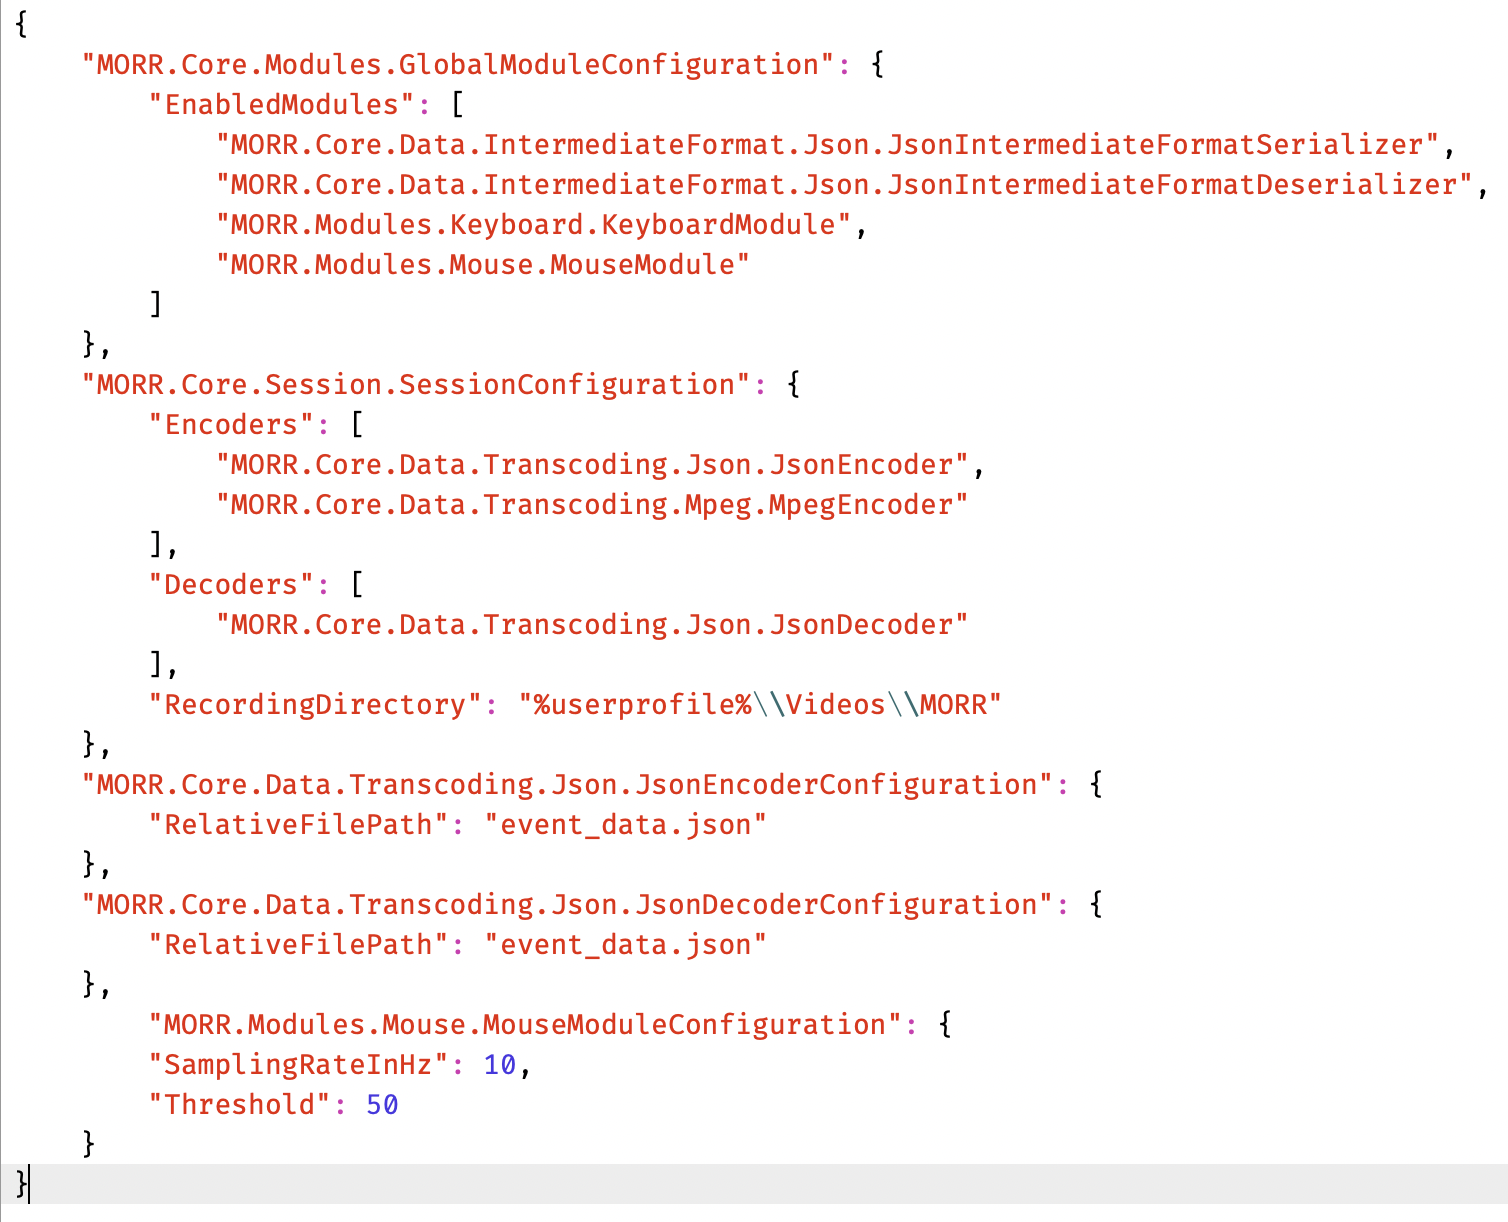
\includegraphics[width=0.8\linewidth]{resources/ConfigExample.png}
   \end{frame}
\end{document}